\documentclass[12pt,a4paper]{article}
\usepackage[top=25.4mm, bottom=25.4mm, left=19.1mm, right=19.1mm]{geometry}


\usepackage[latin2]{inputenc}
\usepackage{graphicx}
\graphicspath{ {./images/} }
\usepackage{ulem}
\usepackage{amsmath}
\usepackage[document]{ragged2e}

\setlength{\parindent}{4em}
\setlength{\parskip}{1em}
\usepackage{hyperref}

\usepackage{fancyhdr}
\pagestyle{fancy}
\fancyhf{}
\fancyhead[LO]{\textbf{\small IoT and Smart Analytics}\\
\text{\small A Program by IIITH and TalentSprint}}

\usepackage{xcolor}
\usepackage{lipsum}

\rhead{\begin{picture}(0,0) \put(-250,-2){
\includegraphics[width=9cm]{EXP_08_Images/ts-iisc-logo-pr.png}} \end{picture}}
\cfoot{\thepage}


\begin{document}

\begin{center}

\textbf{\large \\EXPERIMENT 08 }\\[6pt]
\text{Arduino Interfacing with Stepper and Servo Motor  }
\end{center}

\textbf{\large LEARNING OBJECTIVES:}\\[3pt]
At the end of this experiment, participants will be able to:\vspace{-6mm}\begin{enumerate}
 \setlength\itemsep{-0.3em}
\item Connect \& use Stepper Motor with Arduino \\
\item Connect \& use Servo Motor  with Arduino 
\end{enumerate}
\textbf{\large APPARATUS REQUIRED:}\\
\vspace{-3mm}
\begin{enumerate}
 \setlength\itemsep{-0.3em}
\item Arduino Module-1pcs \\
\item USB cable-1pcs\\
\item DC-DC Voltage Converter Power Supply Module-1pcs\\
\item Stepper Motor (28YBJ-48)-1pcs\\
\item Stepper Motor Driver Board (ULN2003)-1pcs\\
\item Servo Motor (MG995)-1pcs\\
\item Breadboard-1pcs\\
\item Jumper wires\\
\item Arduino IDE
\end{enumerate}

\begin{justify}
\textbf{\large THEORY}\\[3pt]
\textbf{Stepper Motor}: A unipolar stepper motor (available in our kit) consists of two coils, with each coil having a center tap resulting in three connections on each coil. The two center taps are internally connected, and only five leads remain for connections, shown in the figure below.

\begin{center} 
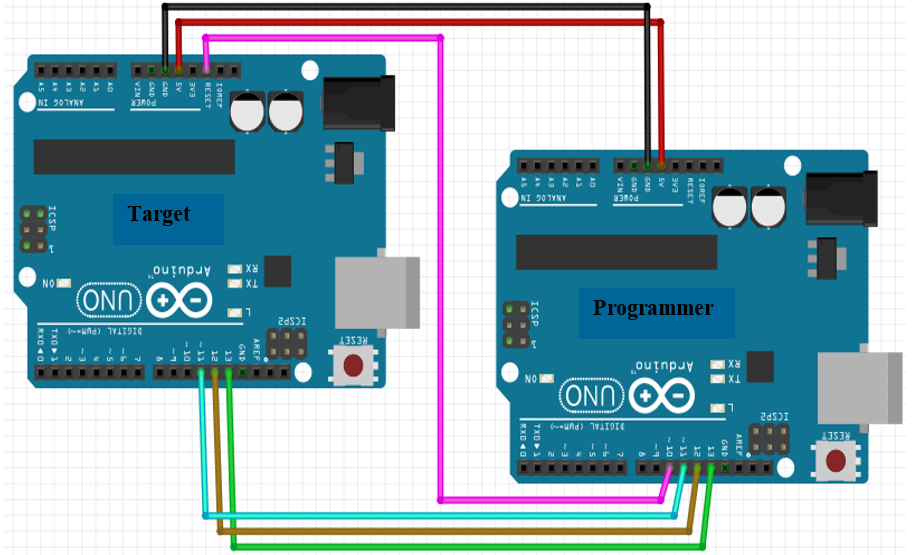
\includegraphics[scale=0.5]{EXP_08_Images/fig1.png}
\end{center}

\begin{center} {Figure 1. Bipolar Stepper Motor Coils
connections}\end{center}
Bipolar stepper motors consist of two coils ( may be split into several physical coils) and have four connections, two per coil. Fig.1 without the centre tap can be seen as a bipolar stepper motor.\par 
\noindent The motor shaft can be moved in discrete steps by controlling the current flowing through the four 
coils: blue, pink, yellow and orange (shown in the figure above). Similarly, the clockwise/anticlockwise direction of rotation is achieved by changing the sequence of coil firing.
Table 1. below shows the different modes of operation with their characteristics and firing orders/steps. 
The same step angle can be achieved using both Wave driving and Full stepping, but the latter has a 
torque twice that of Wave driving. The higher torque is achieved in the Full stepping mode because 
two phases are energized at any one given time step. Half-stepping mode is more precise than Full 
stepping mode since we can get half step angle compared to Full stepping mode, but the torque is lower 
than Full stepping mode.

\begin{center} {Table 1. Mode of operation \& corresponding firing order in Stepper Motor[1]}\end{center}

\begin{center} 
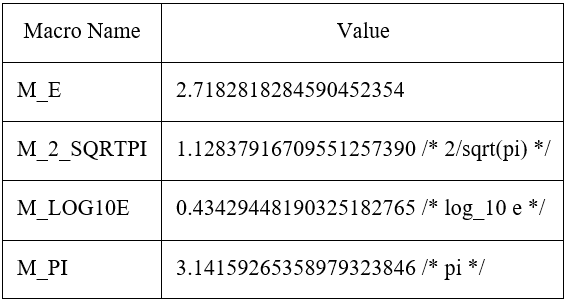
\includegraphics{EXP_08_Images/table1.png}
\end{center}
Stepper motors have a step angle.The number of steps per revolution is given by dividing the full 360° 
circle by the step angle. For example, 1.8° per full step is a common step size rating, which is 
equivalent to 200 steps per revolution. Step angle can be calculated using the data sheet. \\
\textbf{Servo Motor:} A Servo Motor is a low-speed, high-torque motor that can spin up to a limited range 
of 180, 270, or 90 degrees. It contains a motor, a feedback circuit, and, most importantly, a motor 
driver as one package. It provides three terminals for connection: one power line (Red-colored wire), 
one ground (Black/Brown), and one control pin (Yellow or White ). The signal required to move the 
motor arm to a desired position is obtained from the arduino using just one pin (control pin). The 
signal is a square wave similar to PWM. Each cycle in the signal lasts for 20 milliseconds, i.e., having 
a frequency of 50 Hz.Different positions can be achieved by changing the width of the HIGH signal, as shown in the figure 
below.


\begin{center} 
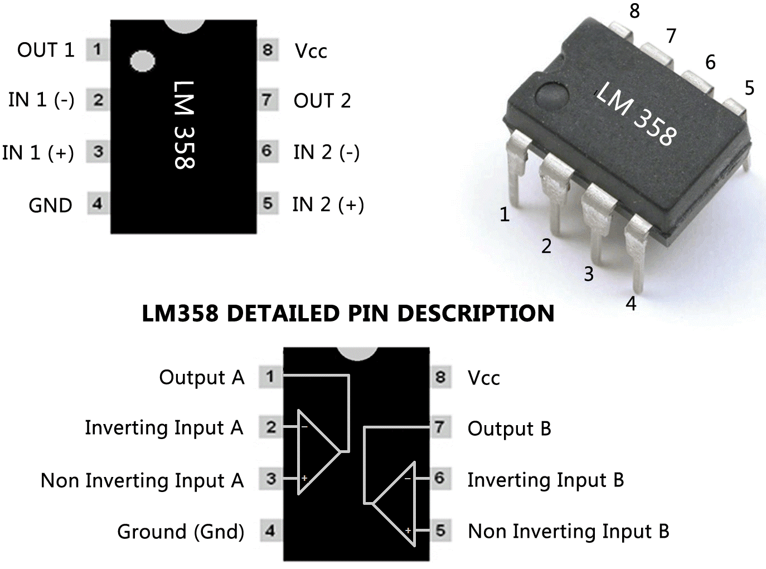
\includegraphics[scale=0.9]{EXP_08_Images/fig2.png}
\end{center}

\begin{center}Figure 2. PWM signals for different positions of Servo Motor arm[2]\end{center}
\vspace{-5mm}
Note that the pulse width can vary slightly for getting different positions of motor arm based on types and brands of servo motors. It is better to try in the range of 0.5 to 2.5 ms.\\[21pt]\textbf{\large PROCEDURE}\\[3pt]
\textbf{(A)	Interfacing Stepper Motor with Arduino}\\[3pt]
\textbf{Hardware and software setup :} The fig. below shows the circuit connection with the required component for the interfacing of the Stepper Motor with Arduino. A stepper driver module (ULN2003) is used in between the motor and Arduino, which is supplied by an external power source: DC-DC Voltage Converter Power Supply Module. Software setup remains as usual, and we are going to write a program without using a built-in library to get a clear understating of its functionality. Following the firing order, as given in table 1, a program is developed for the Full step mode of operation and functions are written for getting clockwise and anticlockwise rotation. The user can put the desired angle of rotation. Note the step angle is 0.72 degrees for the given stepper motor.\end{justify}


\begin{center} 
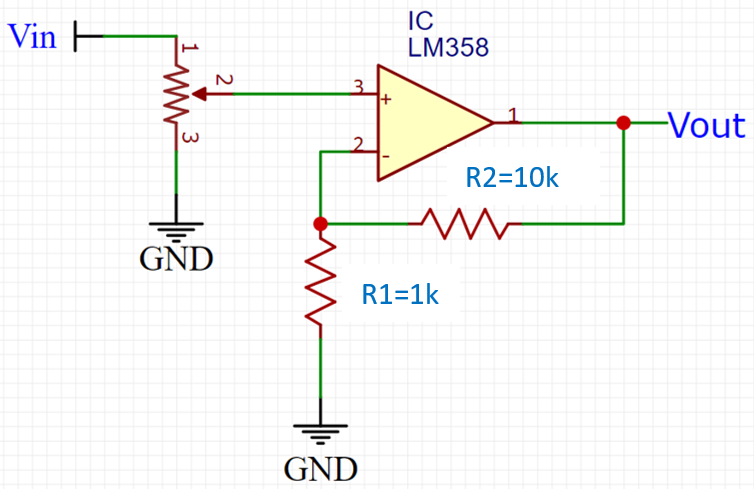
\includegraphics{EXP_08_Images/fig3.PNG}
\end{center}

\begin{center} {Figure 3. Interfacing Stepper Motor with Arduino}\end{center}

\hspace{2cm}\textbf{\large Code:}\\[6pt]

\textcolor{blue}{// Defining supply pins for coil terminals of the Stepper Motor, kept in firing order for clockwise rotation}

\setlength{\parindent}{10eM}

\#define blue     11\\
\#define pink     10\\           
\#define yellow   9\\                        
\#define orange   8\\
\#define waiting\_time 5\\[3pt]

\textcolor{blue}{// Increase this time and observe the change in speed}\\[3pt]

 void clockwise() \hspace{12pt}\textcolor{blue}{//function for clockwise rotation\\}
 \{ \\       
  digitalWrite(blue, HIGH);\\
  digitalWrite(pink, HIGH);\\
  digitalWrite(yellow, LOW);\\
  digitalWrite(orange, LOW);\\
  delay(waiting\_time);\\[3pt]

  digitalWrite(blue, LOW) ;\\
  digitalWrite(pink, HIGH);\\
  digitalWrite(yellow, HIGH);\\
  digitalWrite(orange, LOW);\\
  delay(waiting\_time);\\[3pt]

  digitalWrite(blue, LOW) ;\\
  digitalWrite(pink, LOW);\\
  digitalWrite(yellow, HIGH);\\
  digitalWrite(orange, HIGH);\\
  delay(waiting\_time);\\[3pt]

  digitalWrite(blue, HIGH) ;\\
  digitalWrite(pink, LOW);\\
  digitalWrite(yellow, LOW);\\
  digitalWrite(orange, HIGH);\\
  delay(waiting\_time);\\
  
 \}\\

void anticlockwise() \hspace{12pt}\textcolor{blue}{//function for anticlockwise rotation\\}
\{   \\        
  digitalWrite(orange, HIGH);\\
  digitalWrite(yellow, HIGH);\\
  digitalWrite(pink, LOW);\\
  digitalWrite(blue, LOW);\\
  delay(waiting\_time);\\[3pt]

  digitalWrite(orange, LOW) ;\\
  digitalWrite(yellow, HIGH);\\
  digitalWrite(pink, HIGH);\\
  digitalWrite(blue, LOW);\\
  delay(waiting\_time);\\[3pt]

  digitalWrite(orange, LOW) ;\\
  digitalWrite(yellow, LOW);\\
  digitalWrite(pink, HIGH);\\
  digitalWrite(blue, HIGH);\\
  delay(waiting\_time);\\[3pt]

  digitalWrite(orange, HIGH) ;\\
  digitalWrite(yellow, LOW);\\
  digitalWrite(pink, LOW);\\
  digitalWrite(blue, HIGH);\\
  delay(waiting\_time);\\[3pt]
  
 \}\\[3pt]

  void setup() \\
  \{\\
  pinMode(blue, OUTPUT);\\
  pinMode(pink, OUTPUT);\\
  pinMode(yellow, OUTPUT);\\
  pinMode(orange, OUTPUT);\\
\}\\[3pt]

\begin{center}\textcolor{blue}{// Implementation of above function for 90-degrees clockwise rotation followed by anticlockwise rotation}\end{center}
\vspace{20mm}

void loop() \\
\{  \\                  
 for (int i=0;i$<$=90/0.72;i++) \hspace{12pt} \textcolor{blue}{// changeable angle : 90 degrees \\}
 \{  clockwise();  \}\\
  delay(2000);\\

  for (int i=0;i$<$=90/0.72;i++)\\
  \{ anticlockwise(); \}\\
  delay(2000);\\
\}\par

\setlength{\parindent}{0pt}
\begin{justify}
\textbf{(B)	Interfacing Servo Motor with Arduino Arduino}\\[3pt]
{\textbf{Hardware and software setup :}Figure 4. below shows the circuit connection for the interfacing of the Servo Motor with Arduino. The control signal is given through Pin  9 of the Arduino. Two for loops are implemented one for moving in the direction of  desired angle and the second for returning to its initial state. The desired angle of rotation can be achieved by changing the HIGH pulse width as given in fig. 2 and it is controlled by variable d1 in the code given below. There will be no change in the second loop as it always moves back the motor arm to zero degrees, i.e. initial position. The program has been written without using the library available in Arduino for understanding the underlying functionality.}\end{justify}


\begin{center} 
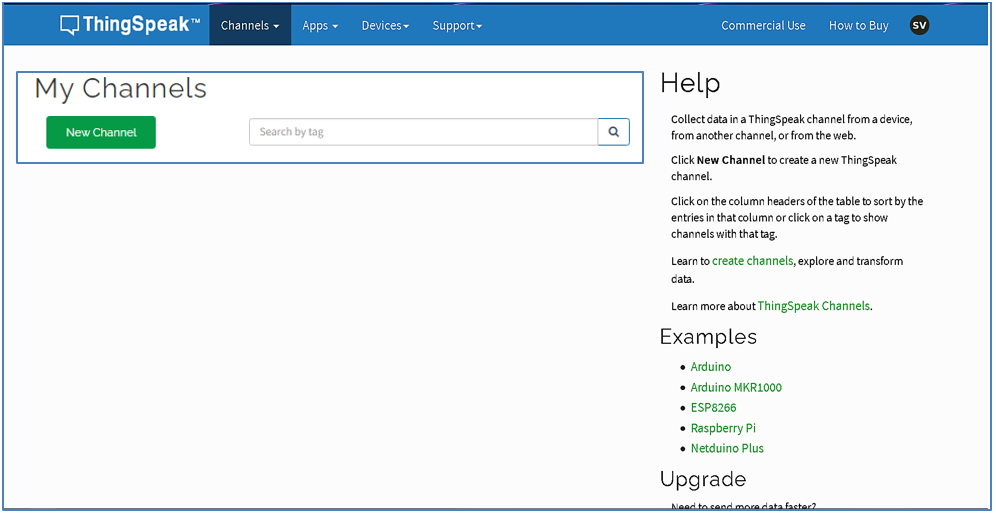
\includegraphics{EXP_08_Images/fig4.png}
\end{center}

\begin{center} {Figure 4. Interfacing Servo Motor with Arduino}\end{center}

\vspace{50mm}

\hspace{2cm}\textbf{\large Code:}\\[6pt]

\setlength{\parindent}{10eM}

float d1;\\
float d2;\\
void setup()\\
\{\\
   d1=1; \textcolor{blue}{//check by putting d1=0.5, 1.5, 2, 2.5}\\
   d2=20-d1; \\
   pinMode(9, OUTPUT);\\
\}\\
void loop()\\
\{\\
  \textcolor{blue}{ // loop for clockwise rotation}\\
   for(int i=0;i$<$=50;i++)\{\\
   digitalWrite(9, HIGH);\\
   delay(d1); \textcolor{blue}{// delay for d1 millisecond(s)}\\
   digitalWrite(9,LOW);\\
   delay(d2);\textcolor{blue}{// delay for d2 millisecond(s)}\\
  \}\\
   delay(3000);\\

  \textcolor{blue}{ // loop for returning back (anticlockwise) to its initial state 0 degree.}\\
   for(int j=0;j$<$=50;j++)\{\\
   digitalWrite(9, HIGH);\\
   delay(0.5);  \textcolor{blue}{// delay for 0.5 millisecond(s)}\\
   digitalWrite(9, LOW);\\
   delay(19.5); \textcolor{blue}{// delay for 19.5 millisecond(s)}\\
   \}\\
   delay(1000);\\
\}\\[21pt]
\setlength{\parindent}{0eM}
\textbf{\large REFERENCES:}
\vspace{-6mm}
\begin{enumerate}
\setlength\itemsep{-0.3em}
 \item  \href{https://www.seeedstudio.com/blog/2019/03/04/driving-a-28byj-48-stepper-motor-with-a-uln2003-driver-board-and-arduino/}{Driving the 28BYJ-48 Stepper motor and ULN2003 Board with an Arduino }
\item   \href{https://www.makerguides.com/servo-arduino-tutorial/}{Pulse train for Servo Motor position control}
\end{enumerate}

\textbf{\large CONCEPT DRILLS:}
\vspace{-6mm}
\begin{enumerate}
 \setlength\itemsep{-0.3em}
\item Design a circuit and write the appropriate program (code) to run the Stepper Motor in half wave drive mode.
\item Operate Stepper motor using \href{https://www.arduino.cc/en/reference/stepper}{Arduino library.}
\item Operate Servo motor using \href{https://www.arduino.cc/reference/en/libraries/servo/}{Arduino library.}
\end{enumerate}
\end{document}